\section{Kuantum Ölçüm Paradoksu, Ölçek-Zaman Kalkülüsü ve Nilpotent Çöküş Mekanizması}
\label{sec:kuantum_olcum_main}

Standart kuantum mekaniğinde dalga fonksiyonunun ($\psi$) deterministik ve lineer Schrödinger evriminden ($i\hbar \partial_t \psi = \hat{H}\psi$), dedektörle temas anında stokastik ve süreksiz bir ``çöküşe'' ($|\psi|^2 \to \delta(\mathbf{x} - \mathbf{x}_0)$) nasıl ve neden sıçradığı çözülememiş bir postulat (Kopenhag yorumu) olarak kalmıştır. Von Neumann ölçüm zincirinin fiziksel bir sınır çizememesi ve Schrödinger dalga denklemi zaman simetrikken ($t \to -t$) ölçüm sürecinin neden mutlak olarak \textbf{geri döndürülemez (irreversible)} olduğu sorusu, bir asırdır modern fiziğin en derin ontolojik krizidir.

Bu bölümde, Birleşik Büzülme Hipotezi ve Ölçek-Zaman Kalkülüsü ($\kappa^2 = 0$, Skalor Uzayı, $\mathbb{D}_t$) çerçevesinde kuantum ölçüm problemini bütünüyle analitik, geometrik ve deterministik bir temele oturtuyoruz. Göstereceğimiz üzere; \textbf{dalga fonksiyonu uzayda yok olup tek bir noktaya çökmez; ölçeksiz statik Öklid uzayındaki kesintisiz bir faz dalgası, sürekli büzüşen atomik bir gözlemcinin ($\kappa$) koordinat sistemine izdüşürüldüğünde zorunlu olarak noktasal bir özdeğer illüzyonu doğurur.}

\subsection{Skalor Ayrışımı: Zamansız Serbest Dalga vs. Büzülen Dedektör}
\label{sec:skalor_ayrisimi}

Bölüm~\ref{sec:olcek_kalkulusu_ana}'da inşa ettiğimiz Ölçek-Zaman Cebirinde bir fiziksel varlığın tam durumu Skalor uzayında tanımlanır:
\begin{equation}
    \mathbb{S}(t) = \mathbf{X}_0 + \kappa \cdot \lambda(t), \quad \kappa^2 = 0.
    \label{eq:skalor_durum_olcum}
\end{equation}
Burada evrendeki iki temel varlık modu arasında kesin bir ontolojik ayrım mevcuttur:
\begin{enumerate}
    \item \textbf{Serbest Dalga (Foton / Dalga Fonksiyonu $\psi$):} Foton, mutlak durağan Öklid sürekliliği ($\mathcal{E}_\infty$) üzerindeki enine elastik bir faz salınımıdır. \textbf{Foton kendi içine büzülmez ($\dot{\lambda} = 0$).} Dolayısıyla fotonun Skalor durumunda nilpotent büzülme bileşeni bulunmaz; foton saf reel statik uzay dalıdır:
          \begin{equation}
              \mathbb{S}_{\mathrm{dalga}} = \mathbf{X}_0 \quad (\kappa = 0 \text{ dalı}).
              \label{eq:foton_skalor}
          \end{equation}
          Ölçek-Zaman Kalkülüsünün en temel teoremi olan Teorem~\ref{thm:zaman_turetilis} uyarınca fiziksel zaman akışı $dt \equiv -\frac{1}{H_0}\frac{d\lambda}{\lambda}$'dir. Büzülmenin olmadığı bir sistemde $d\lambda = 0$ olduğundan \textbf{foton için fiziksel zaman akışı yoktur ($dt = 0$)}. Foton, statik Öklid uzayında zamansız, ölçeksiz, sonsuz uzaya yayılmış deterministik bir faz süperpozisyonudur; bu durum kuantum alan teorisindeki fotonun yerelleşemezliği problemine de doğal bir geometrik zemin sunar~\cite{paul1982}.
    \item \textbf{Gözlemci ve Dedektör (Büzülen Madde):} Dedektör ise durağan vakum dokusunda sürekli kendi içine büzüşen atomik girdaplardan oluşur:
          \begin{equation}
              \mathbb{S}_{\mathrm{det}}(t) = \mathbf{X}_{\mathrm{det}} + \kappa \cdot \lambda(t), \quad \dot{\lambda}(t) = -H_0 \lambda(t).
              \label{eq:dedektor_skalor}
          \end{equation}
          Maddenin içsel ölçeği sürekli daraldığı için ($d\lambda < 0$), dedektörün içsel zaman oku sürekli ileri doğru akar ($dt > 0$).
\end{enumerate}

\subsection{Nilpotent Ölçek İzdüşümü (\texorpdfstring{$\hat{\mathcal{P}}_\kappa$}{P_kappa}) ve Çöküş İllüzyonu}
\label{sec:nilpotent_izdusum}

Kopenhag yorumunun metafizik bir sıçrama saydığı ``ölçüm'', Ölçek-Zaman Kalkülüsünde \textbf{ölçeksiz Öklid fazının, büzülen bir referans çerçevesine ($\kappa$) izdüşürülmesidir (Conformal Scale Projection)}:
\begin{definition}[Nilpotent Ölçüm İzdüşümü]
    \label{def:nilpotent_olcum}
    Statik Öklid uzayında yayılan serbest dalga $\Psi(\mathbf{X}_0)$ ile büzülen dedektör $\mathbb{S}_{\mathrm{det}}$ arasındaki etkileşim, nilpotent projeksiyon operatörü $\hat{\mathcal{P}}_\kappa$ ile tanımlanır:
    \begin{equation}
        \hat{\mathcal{P}}_\kappa : \Psi(\mathbf{X}_0) \longrightarrow \psi_{\mathrm{yerel}}(\mathbf{x}) \ket{\mathbf{x}_0}.
        \label{eq:izdusum_operatoru}
    \end{equation}
\end{definition}

$\kappa^2 \equiv 0$ nilpotent cebrinin ve büzülen referans çerçevesinin en çarpıcı fiziksel sonucu şudur:
Statik uzayda kesintisiz yayılan geniş bir faz dalgası, büzülen atomik bir dedektörle ($\kappa$) inelastik rezonansa girdiği anda, enerji transferi bütünüyle o atomun yerel büzülme sınırında gerçekleşir. İkinci mertebe ölçek etkileşimleri nilpotent cebrin doğası gereği söner ($\kappa^2 \equiv 0$); dedektörün koordinat çerçevesinde serbest faz sürekliliği kopar ve dalga o atomun kendi büzülme sınırına kilitlenir:
\begin{equation}
    \hat{\mathcal{P}}_\kappa : \lim_{\mathrm{etkilesim}} \Delta x_{\mathrm{dalga}} \to r_{\mathrm{atom}}(t).
    \label{eq:nilpotent_sonum}
\end{equation}
Böylece geniş dalga profili, geometrik kesitini aşan rezonant bir absorpsiyon havzası üzerinden~\cite{bohren1983} büzülen ölçüm aygıtının koordinatlarında tekil ve noktasal bir parçacık olarak tecelli eder.

\begin{theorem}[Çöküş İllüzyonu ve Perspektif İzdüşümü]
    \label{thm:cokus_illuzyonu}
    Dalga fonksiyonu uzayda fiziksel olarak tek bir noktaya büzülmez. Gözlemci ölçümü sürekli kendi içine büzülen bir atomik cetvelle ($\lambda(t) \to 0$) gerçekleştirdiği için, durağan Öklid zemininde kesintisiz duran sonsuz faz dalgası, daralan koordinat penceresinden bakıldığında zorunlu olarak tekil bir noktasal parçacık (\textit{Phase-Pinning}) olarak algılanır:
    \begin{equation}
        \lim_{\lambda(t) \to 0} \mathbf{R}_{\mathrm{obs}}(t) = \frac{\mathbf{X}_0}{\lambda(t)} \implies \Delta x_{\mathrm{yerel}} \to r_{\mathrm{atom}}(t).
        \label{eq:cokus_perspektif}
    \end{equation}
\end{theorem}

\subsection{Kuantum Ölçümündeki Geri Dönüşsüzlüğün (Arrow of Time) Gerçek Kökeni}
\label{sec:geri_donussuzluk_zamani}

Standart kuantum teorisinin bir asırdır yanıtlayamadığı en büyük muamma şudur: \textit{``Schrödinger dalga denklemi zaman simetrik ($t \to -t$) olduğu halde, ölçüm anındaki dalga çöküşü neden zamanda asla geriye döndürülemez?''}

Ölçek-Zaman Kalkülüsünde bu sorunun yanıtı son derece berraktır:
\begin{enumerate}
    \item Teorem~\ref{thm:zaman_turetilis}'te ispatlandığı üzere, doğadaki fiziksel zaman oku ($dt > 0$), maddenin vakum gradyanı boyunca büzülmesinin ($\dot{\lambda} < 0$) doğrudan sonucudur. Madde kendiliğinden genişleyemez veya anti-büzüşemez.
    \item Foton serbest vakumda ilerlerken büzülmediği için zamansızdır ($dt_{\mathrm{foton}} = 0$).
    \item Ancak fotonun fazı dedektörün büzüşen bir atomu tarafından soğurulduğu anda, fotonun dalga cephesi \textbf{o atomun yerel büzülme günlüğüne ($dt > 0$) mühürlenir!}
    \item Atomik büzülme tersine çevrilemez bir kozmik olgu olduğundan ($\dot{\lambda} < 0$), \textbf{ölçüm süreci de zamanda mutlak olarak geri döndürülemez!}
\end{enumerate}
Kuantum çöküşündeki geri dönüşsüzlük termodinamik bir kaza değil; evrenin tek yönlü büzülme motorunun doğrudan bir sonucudur.

\begin{figure}[h!]
    \centering
    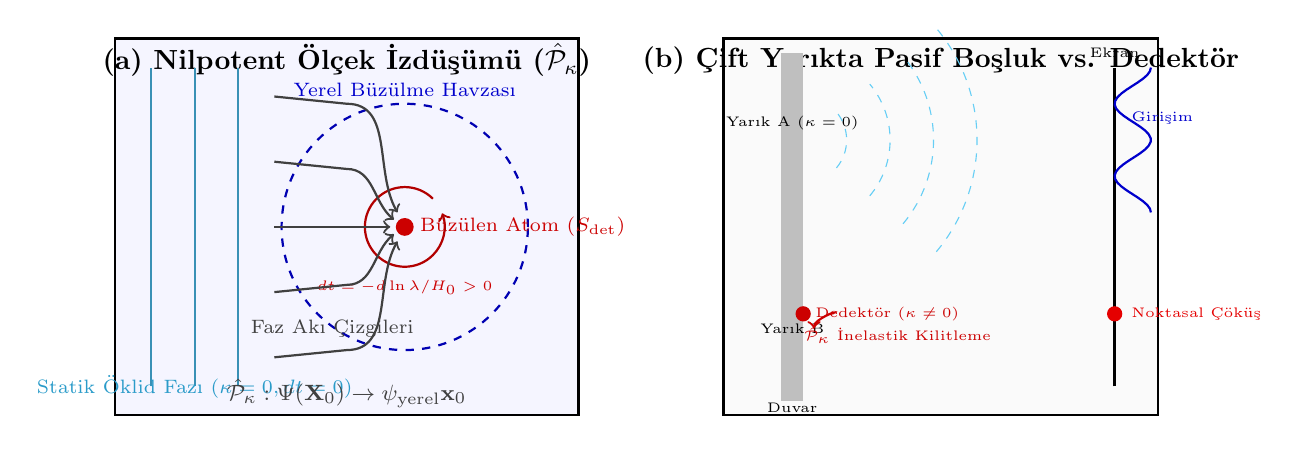
\begin{tikzpicture}[scale=0.92]
        % Panel A: Scale Projection
        \begin{scope}[shift={(-4.4,0)}]
            \draw[thick, fill=blue!4] (-3.2,-2.6) rectangle (3.2,2.6);
            \node at (0, 2.3) {\textbf{(a) Nilpotent Ölçek İzdüşümü ($\hat{\mathcal{P}}_\kappa$)}};

            % Static plane waves in E_infinity
            \foreach \x in {-2.7, -2.1, -1.5} {
                    \draw[cyan!70!black, thick] (\x, -2.2) -- (\x, 2.2);
                }
            \node[cyan!80!black, above] at (-2.1, -2.5) {\scriptsize Statik Öklid Fazı ($\kappa=0, dt=0$)};

            % Resonant cross section boundary
            \draw[dashed, blue!70!black, thick] (0.8,0) circle (1.7);
            \node[blue!80!black] at (0.8, 1.9) {\scriptsize Yerel Büzülme Havzası};

            % Atom vortex sink
            \fill[red!80!black] (0.8,0) circle (3.5pt) node[right=2pt] {\scriptsize Büzülen Atom ($\mathbb{S}_{\mathrm{det}}$)};
            \draw[red!70!black, thick, ->] (0.8,0) ++(45:0.55) arc (45:380:0.55);
            \node[red!80!black, below] at (0.8, -0.6) {\tiny $dt = -d\ln\lambda/H_0 > 0$};

            % Streamlines converging to atom
            \draw[thick, darkgray, ->] (-1.0, 1.8) -- (0.0, 1.7) to[out=0, in=120] (0.7, 0.2);
            \draw[thick, darkgray, ->] (-1.0, 0.9) -- (0.0, 0.8) to[out=0, in=140] (0.65, 0.1);
            \draw[thick, darkgray, ->] (-1.0, 0.0) -- (0.6, 0.0);
            \draw[thick, darkgray, ->] (-1.0, -0.9) -- (0.0, -0.8) to[out=0, in=-140] (0.65, -0.1);
            \draw[thick, darkgray, ->] (-1.0, -1.8) -- (0.0, -1.7) to[out=0, in=-120] (0.7, -0.2);
            \node[darkgray] at (-0.2, -1.4) {\scriptsize Faz Akı Çizgileri};
            \node[darkgray] at (0, -2.3) {\footnotesize $\hat{\mathcal{P}}_\kappa : \Psi(\mathbf{X}_0) \to \psi_{\mathrm{yerel}} \ket{\mathbf{x}_0}$};
        \end{scope}

        % Panel B: Double Slit
        \begin{scope}[shift={(3.8,0)}]
            \draw[thick, fill=gray!4] (-3.0,-2.6) rectangle (3.0,2.6);
            \node at (0, 2.3) {\textbf{(b) Çift Yarıkta Pasif Boşluk vs. Dedektör}};

            % Barrier with two slits
            \fill[gray!50] (-2.2, 1.1) rectangle (-1.9, 2.4);
            \fill[gray!50] (-2.2, -1.1) rectangle (-1.9, 1.1);
            \fill[gray!50] (-2.2, -2.4) rectangle (-1.9, -1.1);
            \node at (-2.05, -2.5) {\tiny Duvar};

            % Slit A: Pure vacuum, elastic propagation
            \node[above] at (-2.05, 1.2) {\tiny Yarık A ($\kappa=0$)};
            \foreach \r in {0.6, 1.2, 1.8, 2.4} {
                    \draw[cyan!60, dashed] (-1.9, 1.2) ++(-40:\r) arc (-40:40:\r);
                }

            % Slit B: Detector with inelastic absorption
            \node[below] at (-2.05, -1.2) {\tiny Yarık B};
            \fill[red!80!black] (-1.9, -1.2) circle (3pt) node[right=1pt] {\tiny Dedektör ($\kappa \neq 0$)};
            \draw[red!80!black, thick, ->] (-1.5, -1.2) to[out=30, in=90] (-1.75, -1.4);
            \node[red!80!black] at (-0.6, -1.5) {\tiny $\hat{\mathcal{P}}_\kappa$ İnelastik Kilitleme};

            % Detection Screen
            \draw[very thick, black] (2.4, -2.2) -- (2.4, 2.2);
            \node[above] at (2.4, 2.2) {\tiny Ekran};

            % Localized spot vs fringe
            \draw[thick, blue!80!black, domain=-1.0:1.0, samples=40] plot ({2.4 + 0.5*(cos(\x*180)^2)}, {\x + 1.2});
            \node[blue!80!black, right] at (2.5, 1.5) {\tiny Girişim};
            \fill[red!90!black] (2.4, -1.2) circle (3pt);
            \node[red!90!black, right] at (2.5, -1.2) {\tiny Noktasal Çöküş};
        \end{scope}
    \end{tikzpicture}
    \caption{\textbf{(a)} Statik Öklid zeminindeki zamansız faz dalgasının ($\kappa=0$), büzülen dedektör çerçevesine nilpotent izdüşümü ($\hat{\mathcal{P}}_\kappa$). \textbf{(b)} Çift yarıkta pasif yarıkların saf Öklid vakumu ($\kappa=0$) olarak faz tutarlılığını koruması, dedektörün ise inelastik $\kappa$-izdüşümüyle dalgayı yerel büzülme merkezine kilitlemesi (\textit{phase-pinning}).}
    \label{fig:skalor_olcum_cift_yarik}
\end{figure}

\subsection{Çift Yarık Deneyi: Neden Duvar Çökertmez de Dedektör Çökertir?}
\label{sec:cift_yarik_cozum}

Burada kritik soru şudur: \textit{``Çift yarığın açıldığı duvardaki atomlar da büzülmektedir. Neden duvarın atomları dalgayı çökertmezken, yarığa konulan dedektör dalgayı bozar ve noktasal parçacığa çökertir?''}

Bu ayrım, Skalor uzayındaki elastik sınır şartı ile inelastik durum transferi arasındaki farktan doğar:
\begin{enumerate}
    \item \textbf{Yarıklar ve Duvar (Elastik Sınır Şartı):} Yarığın kenarındaki atomlar gelen dalgayla rezonansta değildir; durum değiştirmezler ($\Delta E = 0$). Yarığın içi ise hiçbir atom barındırmayan \textbf{saf Öklid vakumudur ($\kappa = 0$)}. Dalga yarıklardan geçerken yalnızca geometrik bir sınır şartını takip eder. Herhangi bir inelastik $\kappa$-izdüşümü gerçekleşmediği için Huygens prensibi gereği iki yarıktan çıkan dalgacıklar arasındaki faz tutarlılığı eksiksiz korunur ve ekranda klasik girişim saçakları oluşur:
          \begin{equation}
              I(\theta) = 4 I_0 \cos^2\left( \frac{\pi d \sin\theta}{\lambda} \right).
              \label{eq:girisim_sacagi_main}
          \end{equation}
    \item \textbf{Yarıktaki Dedektör (İnelastik $\kappa$-İzdüşümü):} Yarıklardan birine yerleştirilen dedektör, ``foton buradan geçti mi?'' sorusunu yanıtlayabilmek için dalgadan inelastik olarak tam $\hbar\omega$ çeker. Faz, dedektör atomunun içsel durumuna devredildiği anda ($\hat{\mathcal{P}}_\kappa$), o koldaki dalga cephesinin vakumdaki serbest faz bağı kopar (inelastik dekoherens). İki yarık arasındaki faz korelasyonu yok olduğu için ekrandaki girişim saçakları silinir ve geriye yalnızca iki bağımsız şiddet dağılımının toplamı kalır:
          \begin{equation}
              I_{\mathrm{toplam}} = I_1 + I_2.
              \label{eq:klasik_toplam}
          \end{equation}
\end{enumerate}

\subsection{Bell Teoremi ve Boşluğun Parçalanamaz Bütünlüğü}
\label{sec:bell_ve_nonlokalite}

Modelimiz yerel gizli değişkenler teorisi değildir. Mutlak durağan Öklid sürekliliği $\mathcal{E}_\infty$, piksellenemez ve parçalanamaz tekil bir bütündür. Dolanık iki foton uzayda keyfi mesafelere ayrılsa dahi, aralarındaki vakum faz sürekliliği bölünmez bir potansiyel oluşturur. Clauser, Aspect ve Zeilinger deneyleriyle kanıtlanan kuantum holizmi, Bell eşitsizliklerinin ihlali ve kuantum silgisi korelasyonları~\cite{scully1982,kim2000}; ışıktan hızlı gizli parçacık sinyallerinden değil, \textbf{arka plan vakumunun ayrık piksellerden değil, kesintisiz bir süreklilikten ibaret olmasından} kaynaklanır. Kuantum ölçüm mekaniğinin genişletilmiş analitik temelleri için külliyatımızın Makale~II çalışmasına~\cite{haydari_calculus} başvurulmalıdır.
